\section{Decision trees}

\begin{enumerate}
\item Concrete sample training data.
  \begin{enumerate}
  \item The sample entropy $H(Y)$ is $0.985$.
    \begin{align*}
      H(Y)= & \;-p(y=+)\log(p=+)-p(y=-)\log p(y=-)\\
= & \;-4/7\log4/7-3/7\log3/7\\
= & \;0.985
    \end{align*}

  \item The information gains are $IG(X_1) = 0.183$ and $IG(X_2) = 0.045$.  
    \begin{align*}
      IG(X_{1})= & \; H(y)-H(y|x_{1})\\
= & \; H(y)-(-7/21\log7/8-1/21\log1/8-5/21\log5/13-8/21\log8/13)\\
= & \;0.985-0.802=0.183\\
IG(X_{2})= & \; H(y)-H(y|x_{2})\\
= & \; H(y)-(-7/21\log7/10-3/21\log3/10-5/21\log5/11-6/21\log6/11)\\
= & \;0.985-0.940=0.045
    \end{align*}

  \item The decision tree that would be learned is shown in Figure
    \ref{fig:decision_tree}.
    %% The [H], in combination with the float package, forces latex to
    %% generate the figure in exactly this part of the document
    %% instead of ``floating'' it to another part.
    \begin{figure}[H]
      \centering
      \tikzstyle{dir}=[->, very thick]
      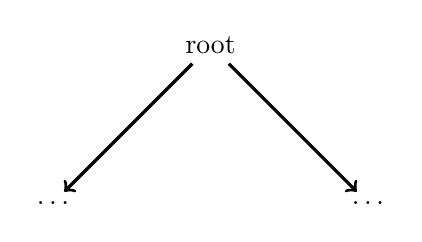
\begin{tikzpicture}[auto]
        \node[rectangle] (root) at (0,0) {root};
        \node (left) at (-2,-2) {$\ldots$};
        \node (right) at (2,-2) {$\ldots$};

        \draw[dir] (root) to [above] node {} (left);
        \draw[dir] (root) to [above] node {} (right);
      \end{tikzpicture}
      \caption{The decision tree that would be learned.}
      \label{fig:decision_tree}
    \end{figure}
  \end{enumerate}

\item Proof that $IG(x,y) = H[x] - H[x \mid y] = H[y] - H[y \mid x]$,
  starting from the definition in terms of KL-divergence:
  \begin{align*}
    IG(x,y)= & \; KL\left(p(x,y)||p(x)p(y)\right)\\
= & \;-\sum_{x}\sum_{y}p(x,y)\log(\frac{p(x)p(y)}{p(x,y)})\\
= & \;-\sum_{x}\sum_{y}p(x,y)\log p(x)+\sum_{x}\sum_{y}p(x,y)\log(\frac{p(x,y)}{p(y)})\\
= & \;-\sum_{x}p(x)\log p(x)-(-\sum_{x}\sum_{y}p(x,y)\log p(x|y))\\
= & \; H[x]-H[x\mid y]
    \end{align*}
\end{enumerate}
